% =====================================================================
% Paper 1 --- Common-random-number ablation of architectures and vehicle
% response channels for multi-pier railway-bridge scour monitoring
%
% Venue: TBD (structure follows Fernandes et al. 2025, IJSSD).
% Status: PRE-RESULTS DRAFT. The four-block Paper-1 campaign has not run;
% every result placeholder is marked \pending{...}. Do NOT import pilot,
% retired-rung, or pre-freeze numbers.
% Controlling source: docs/paper1_campaign_plan.md, together with the
% authorized source commit and authenticated campaign artifacts.
% =====================================================================
\documentclass[11pt]{article}
\usepackage[utf8]{inputenc}
\usepackage[T1]{fontenc}
\usepackage{authblk}
\usepackage{setspace}
\usepackage[margin=1.25in]{geometry}
\usepackage{graphicx}
\graphicspath{{./figures/}}
\usepackage{subcaption}
\usepackage{amsmath}
\usepackage{amssymb}
\usepackage{booktabs}
\usepackage{multirow}
\usepackage{siunitx}
\usepackage{xcolor}
\usepackage{tikz}
\usetikzlibrary{positioning,arrows.meta}
\usepackage{lineno}
\usepackage[hidelinks]{hyperref}
\linenumbers

% ---------------------------------------------------------------------
% Draft-status macros (remove before submission)
% \pending{...} : value/claim that exists only after the authenticated
%                 four-block campaign; never replace with a pilot value.
% \verifyref{...}: citation whose bibliographic data still needs a
%                 primary-source check.
% ---------------------------------------------------------------------
\newcommand{\pending}[1]{\textcolor{red!70!black}{[\textbf{PENDING RESULTS:} #1]}}
\newcommand{\verifyref}[1]{\textcolor{blue!60!black}{[verify: #1]}}

%%%%%% Bibliography %%%%%%
\usepackage[backend=biber,style=numeric-comp,sorting=none,maxbibnames=8]{biblatex}
\addbibresource{references.bib}
% Allow DOIs/URLs to break in the bibliography
\setcounter{biburlnumpenalty}{100}
\setcounter{biburlucpenalty}{100}
\setcounter{biburllcpenalty}{100}

%%%%%% Title %%%%%%
\title{Common-Random-Number Ablation of Architectures and Vehicle Response
Channels for Multi-Pier Railway-Bridge Scour Monitoring}
% Alternative title (adopt only if authenticated results justify it):
% Drive-by estimation of multi-pier support-stiffness loss under competing
% bridge damage mechanisms

%%%%%% Authors %%%%%%
\author[1,2*]{Gabriel Padilha Alves}
% \author[2]{Co-author TBD}
\affil[1]{Department of Civil Engineering, Federal University of Santa
Catarina, Florian\'opolis, Brazil}
\affil[2]{Department of Structural Engineering, University of California
San Diego, La Jolla, CA, USA}
\affil[*]{Address correspondence to: gpadilhaalves@gmail.com}

\date{\today}

\onehalfspacing

\begin{document}

\maketitle

%%%%%% Abstract %%%%%%
\begin{abstract}
% NOTE: single paragraph, plain language, no citations. Target 200--250 words.
% The two \pending sentences must be rewritten with observed effect sizes after
% the authenticated four-block campaign; do not soften the pending markers.
Scour --- the erosion of soil around bridge foundations during floods --- is a
leading cause of bridge failure, yet it is difficult to inspect exactly when it
matters most. Drive-by monitoring offers an attractive alternative: an
in-service train records its own vibration while crossing the bridge, and that
response carries information about support condition. Previous studies
established feasibility but leave pre-deployment choices unresolved:
whether to process raw or compressed signals, which neural components help,
and which response channels are informative. This study addresses
those questions with a prospectively specified, source-locked experiment based
on a two-dimensional train--track--bridge simulation of a two-span benchmark
and a four-span geometry. Four blocks separate scour
from a multi-damage task that activates nominal bearing fixity and a local
flexural-rigidity-loss surrogate. One fixed rail-profile realization is shared
throughout; speed, temperature, and vehicle properties vary between passages,
while track damage, wheel polygonization, and suspension damage are deferred.
A 16-cell factorial compares raw and Piecewise Aggregate Approximation inputs,
positional encoding, recurrence, and fixed-width multi-rate pooling. A sealed,
state-grouped protocol then screens all eight single channels descriptively and
all 28 two-channel pairs for four retained pipelines. The eight modeled inputs
include two constrained-wheelset acceleration proxies and therefore represent
responses, not a validated eight-sensor package.
\pending{State the authenticated RAW/PAA factorial and selected-pair outcomes,
with effect sizes and explicitly descriptive finite-design uncertainty.}
\pending{State the authenticated block-local scour, multi-damage, and
multi-pier results without importing pilot or pre-freeze values.} The resulting
workflow provides an auditable template for simulation-based design decisions
before field validation.

\end{abstract}

\noindent\textbf{Keywords:} drive-by monitoring; bridge scour; train--track--bridge
interaction; deep learning; ablation study; common random numbers; railway bridges

\section{Introduction}
\label{sec:introduction}

\subsection{Motivation}
\label{sec:motivation}

Scour --- the removal of riverbed material from around bridge foundations by
flowing water --- is consistently identified as a leading cause of bridge
failure~\cite{wardhana2003analysis, arneson2012hec18}. For railway networks the
exposure is systemic: a single scour-critical crossing can close a line, and
probabilistic assessments of the British railway network attribute a
substantial share of its weather-related risk to bridge scour during
floods~\cite{lamb2019scour}. The hazard is also awkwardly timed. Scour develops
fastest during high flows, exactly when visual and diver inspections are most
dangerous and least reliable, and damage can refill with loose sediment before
an inspection takes place~\cite{prendergast2014review, arneson2012hec18}.
Instrumenting every vulnerable bridge permanently is rarely economical for a
large inventory, which motivates indirect approaches that reuse vehicles
already crossing the structure.

Drive-by monitoring extracts information about a bridge from the dynamic
response of a traversing vehicle, an idea introduced for bridge-frequency
identification by Yang et al.~\cite{yang2004extracting} and since developed
into a broad research field~\cite{malekjafarian2015review}, including dedicated
railway applications~\cite{braganca2023review, souza2023review}. The physical
basis for drive-by scour monitoring is established: foundation-stiffness loss
changes the soil--foundation and structural dynamics
\cite{prendergast2013investigation, prendergast2016determining}. Wavelet-based
analyses of simulated train-borne signals identified localized scour
signatures~\cite{fitzgerald2019drive}; vehicle pitch has shown specific scour
sensitivity~\cite{mcgeown2024pitch}; scour-induced stiffness loss has been
identified from field-measured drive-by data~\cite{tola2025scour}; and
machine-learning pipelines have classified scour severity under operational
variability~\cite{fernandes2024driveby, fernandes2025early,
fernandes2026early, fernandes2026canelas}. A vehicle-borne estimate of
foundation condition is also a natural input to decision-oriented monitoring
and digital-twin frameworks~\cite{kamariotis2023framework,
torzoni2024digital}, which benefit from a continuous component-level state
rather than a binary alarm.

\subsection{Related work: the drive-by scour and multi-damage line}
\label{sec:related}

This study continues the drive-by scour programme developed by Fernandes and
co-workers. Fernandes et al.~\cite{fernandes2024driveby} detected scour,
modeled as local pier-foundation stiffness loss, with an unsupervised deep
autoencoder operating on raw vertical accelerations. Comparing on-board
positions, they found the best detection at the bogies. Fernandes et
al.~\cite{fernandes2025early} then studied supervised multi-damage
classification of cracks, bearing-device damage, and scour using min--max
normalization, Piecewise Aggregate Approximation (PAA), and a CNN tuned by
Bayesian optimization. Fernandes et al.~\cite{fernandes2026early} classified
scour levels with a supervised CNN and showed the value of adding speed as an
input. Fernandes et al.~\cite{fernandes2026canelas} extended the approach to a
high-fidelity finite-element model of the Canelas railway bridge, calibrated to
field modal parameters, using a Bayesian-optimized CNN--LSTM.

Three wider strands shape the present design. First, drive-by learning studies
often hold the rail-irregularity profile fixed within a scenario while varying
speed, mass, and noise~\cite{locke2020using, fernandes2025early}; profile
handling must therefore be stated as an experimental choice. Second,
sprung-mass channels are filtered by the suspension, whereas unsprung or
axle-level responses act nearer the wheel--rail interface
\cite{molodova2011axle, malekjafarian2015review}, which motivates comparing
responses across suspension levels. Third, two-sensor residual concepts can
cancel shared profile content~\cite{keenahan2014use, obrien2015apparent}, so
pairs may contain information that neither member provides alone.

This literature establishes feasibility, but it does not give a controlled
answer to the linked design choices of representation, neural components, and
response channels. Published studies generally optimize one pipeline or a
small set of preselected positions. Independent searches can also mix method
quality with finite hyperparameter-search luck, while passage-level splitting
can leak the repeated observations of one bridge state across partitions.

\subsection{Gap and design questions}
\label{sec:gap}

The experiment reported here is prospectively specified and source-locked:
its scientific blocks, state catalogues, splits, training grid, selection
rules, and analysis roles were fixed in versioned, hash-identified source
before production data were generated. Throughout this paper, ``registered''
is shorthand for that repository-fixed specification; it denotes no external
registry deposit.

The settled Paper-1 campaign contains four blocks rather than a progressive
mechanism ladder. F40-S is a two-span, one-target scour benchmark; F40-M adds
nominal bearing fixity and local flexural-rigidity loss. L99-S and L99-M repeat
those scour-only and multi-damage roles on a four-span, three-target geometry.
All four blocks use one generated FRA-class-4 profile realization (registered
phase seed 20260728), shared by every state and passage. Speed, temperature,
and vehicle properties vary between passages.
Track-layer damage, wheel polygonization, and suspension damage are deferred by
configuration; their implementation remains in the one qualified source tree,
but they are not part of this experiment.

Within that scope, the study asks:

\begin{itemize}
  \item \textbf{RQ1.} On F40-S, how do RAW versus PAA input, Time2Vec-style
  spatial-coordinate encoding, LSTM recurrence, and fixed-width multi-rate
  pooling affect grouped-development scour error across a matched 16-cell HPO
  factorial?
  \item \textbf{RQ2.} Among the six learning-eligible modeled-DOF responses in
  the eight-response \texttt{physical8\_v1} payload,
  which unordered two-channel pair minimizes the prospectively specified
  aggregate screen score for the retained RAW/PAA pipelines, and what do the
  six non-selectable single-channel diagnostics show?
  \item \textbf{RQ3.} After independent selected-pair HPO in each block, how
  accurately do the retained pipelines estimate one or three support-specific
  stiffness-loss targets and localize the most affected support?
  \item \textbf{RQ4.} On the genuinely shared semantic states, how does the
  combined multi-damage physics/task block (nominal bearing fixity, local $EI$
  loss, and bearing heads) differ from its scour-only counterpart in F40 and
  L99?
  \item \textbf{RQ5.} How stable are the frozen configurations across a
  disjoint post-selection initialization set, and what descriptive change is
  observed when F40-S settings are transferred downstream without retuning?
\end{itemize}

Three claim boundaries apply throughout. The target is modeled vertical
support-stiffness loss, not physical scour-hole depth. The inputs are modeled
response channels, not transducer packages or placements. Specifically, the
two wheelset rows are idealized constrained-motion kinematic diagnostics, not
independent vehicle degrees of freedom or validated axle-box observations, and
they are excluded from every learning and selection input. Finally, each block
receives its own selected-pair HPO for the primary analysis, so cross-block
primary results do not measure frozen-hyperparameter transport.

\subsection{Contributions}
\label{sec:contributions}

The paper contributes the following experimental design and, once populated by
the authenticated campaign, its corresponding estimates:

\begin{enumerate}
  \item a four-block, state-grouped simulation design with explicit semantic
  pairing: a 30-state F40-S/F40-M controlled subset and complete
  475-state L99-S/L99-M pairing, with common random numbers only where those
  identities actually match;
  \item a balanced $2\times2\times2\times2$ architecture factorial covering
  RAW/PAA, spatial encoding, recurrence, and fixed-width multi-rate pooling,
  with five independent 100-trial HPO restarts per F40-S cell;
  \item a complete Option-C adjudication in which the five HPO winners per cell
  are compared on one predeclared three-fold grouped-development OOF partition
  before the outer test is opened;
  \item a prospectively listed \texttt{physical8\_v1} response screen over the
  six eligible, non-selectable singles and all 15 selectable pairs for four
  retained RAW/PAA pipeline slots, with paired initialization seeds and
  authenticated alias deduplication;
  \item an optional secondary contemporary-architecture tier admitted only
  after the F40-S screen, in which every challenger uses the same authenticated
  primary selected pair and no challenger performs its own pair selection;
  \item independent selected-pair HPO and disjoint post-freeze stability fits
  in every scientific block, separating primary block-local performance from a
  secondary frozen-F40-S transfer analysis; and
  \item explicit numerical and observation-model boundaries for the
  support-aligned meshes, inherited track topology and scaling, Rayleigh
  damping policy, and diagnostic-only idealized wheelset response proxies.
\end{enumerate}

Table~\ref{tab:delta} summarizes the relation to the closest prior work.
\pending{Add one sentence after Table~\ref{tab:delta} stating the headline
authenticated four-block outcome.}

\begin{table}[htbp]
\centering
\caption{This study in relation to the drive-by scour line of Fernandes et
al. Prior-work entries summarize the cited primary sources.}
\label{tab:delta}
\footnotesize
\setlength{\tabcolsep}{3pt}
\begin{tabular}{p{2.2cm}p{2.8cm}p{2.8cm}p{3.0cm}p{3.2cm}}
\toprule
Work & Task / mechanisms & Pipeline & Selection & Robustness / analysis \\
\midrule
Fernandes 2024~\cite{fernandes2024driveby} & unsupervised scour detection &
raw signal + deep autoencoder & fixed AE; on-board positions compared & KL
damage index, ROC \\
\addlinespace
Fernandes 2025~\cite{fernandes2025early} & classification of crack + bearing +
scour & min--max + PAA + CNN & Bayesian-optimized CNN; two fixed channels &
confusion matrices, boxplots, EOV sensitivity \\
\addlinespace
Fernandes 2026a~\cite{fernandes2026early} & classification of scour levels &
CNN (+ speed input) & Bayesian-optimized CNN; two fixed channels & confusion
matrices, boxplots \\
\addlinespace
Fernandes 2026b~\cite{fernandes2026canelas} & classification of scour depths
(field-calibrated model) & CNN--LSTM & Bayesian-optimized per channel
configuration & multi-run statistics \\
\addlinespace
\textbf{This work} & \textbf{continuous one-/three-support regression,
localization, and bearing co-estimation in four explicit blocks} &
\textbf{RAW/PAA $\times$ position $\times$ LSTM $\times$ fixed-width
multi-rate factorial} & \textbf{Option-C grouped OOF adjudication; complete
  6-single/15-pair screen; per-block selected-pair HPO} & \textbf{sealed outer
test; disjoint post-freeze stability; authenticated paired-state and secondary
transfer roles} \\
\bottomrule
\end{tabular}
\end{table}

\subsection{Paper organization}

Section~\ref{sec:framework} gives the experimental overview.
Section~\ref{sec:simulation} describes the TTBI model, the four state
catalogues, and active/deferred mechanisms. Section~\ref{sec:data_processing}
details preprocessing, architectures, HPO, adjudication, and response-channel
selection. Section~\ref{sec:results} provides results and discussion;
Section~\ref{sec:limitations} states claim boundaries and practical
feasibility; and Section~\ref{sec:conclusion} concludes.

\section{Proposed framework}
\label{sec:framework}

The study is organized as a prospectively specified, source-locked simulation
experiment: the bridge-state catalogues, active-mechanism scope, model-selection
policy, statistical analyses, and claim boundaries were fixed in versioned,
hash-identified source before production generation. In this paper,
``registered'' means fixed in that repository source; it does not imply deposit
in an external registry. This section gives an overview, while
Sections~\ref{sec:simulation} and~\ref{sec:data_processing} provide the
implementation details.

Three principles govern the experiment.

\paragraph{Explicit scientific blocks and common random numbers.}
The campaign contains four blocks: a two-span scour benchmark (F40-S), its
multi-damage counterpart (F40-M), a four-span multi-pier scour block (L99-S),
and its multi-damage counterpart (L99-M). Named random substreams keyed to
semantic state identifiers make all intended comparisons invariant to row
order and parallel scheduling. F40-S and F40-M share an explicit 30-state
controlled subset; their remaining states are not claimed to be paired.
L99-S and L99-M share the complete 475-state latent design. All four blocks use
one fixed rail-profile realization and vary only the registered operational
conditions between passages. Thus any paired contrast uses only states whose
semantic identities and operational draws are genuinely shared.

\paragraph{Block-local calibration.}
The architecture factorial is calibrated on F40-S using the prospectively
chosen front-bogie vertical-acceleration anchor. Frozen hyperparameters then
support the complete F40-S single- and two-channel screen. After the physical
channel pair is selected, the retained pipelines are re-optimized on that pair
in F40-S and independently in F40-M, L99-S, and L99-M. No block inherits
another block's hyperparameters for its primary result. The earlier
transport/rescue trigger is withdrawn; a separate frozen-F40-S transfer
analysis is retained only as a secondary descriptive analysis.

\paragraph{A selection/report firewall.}
States, never passages, are assigned to train, inner-validation, and sealed
outer-test partitions. Hyperparameter search, the Option-C grouped-development
out-of-fold adjudication, and the response-channel screen use development data
only. The outer test remains unopened until the architecture vectors, selected
pair, block-local hyperparameters, checkpoint policy, and comparator set are
frozen. Post-freeze variability is then estimated with a disjoint,
prospectively listed set of initialization seeds and is report-only.

\subsection{Scientific blocks and estimands}
\label{sec:estimands}

Table~\ref{tab:stages} and Figure~\ref{fig:stage_graph} summarize the campaign.
F40-S is the gating method-development block. Its dense 0--60\% grid supports
continuous regression, while the predeclared \{0, 5, 10, 20\%\} subset gives a
limited classification comparability check with Fernandes et
al.~\cite{fernandes2025early}. F40-M activates nominal bearing fixity and a
local flexural-rigidity-loss surrogate in addition to scour. L99-S estimates
three internal supports on a longer four-span bridge, and L99-M activates the
same multi-damage task there.

The design supports four distinct estimand classes:

\begin{enumerate}
  \item \textbf{F40-S method and channel selection.} Grouped-development
  evidence selects one RAW and one PAA factorial cell, and a prospectively
  specified screen over eight singles and 28 pairs selects one physical
  two-channel input. Singles are descriptive and non-selectable.
  \item \textbf{Block-local primary performance.} The retained RAW/PAA winners
  and their RAW/PAA CNN--GAP baselines receive independent selected-pair HPO in
  every block. Performance on the sealed outer test therefore estimates each
  pipeline under block-local calibration, not hyperparameter transport.
  \item \textbf{Paired damage/task comparisons.} F40-S versus F40-M is
  interpreted only on their 30 shared controlled states; L99-S versus L99-M
  uses the complete shared 475-state inventory. Each comparison jointly
  changes the expressed bearing/crack physics and, where applicable, the
  additional bearing regression heads. It is not an isolated causal effect of
  either mechanism.
  \item \textbf{Scale and transfer observations.} Comparisons between F40 and
  L99 are descriptive geometry/scale observations. The secondary frozen-F40-S
  transfer analysis measures performance under deliberately transported
  settings and cannot replace any block's independently tuned primary result.
\end{enumerate}

\begin{figure}[htbp]
\centering
\resizebox{0.88\textwidth}{!}{%
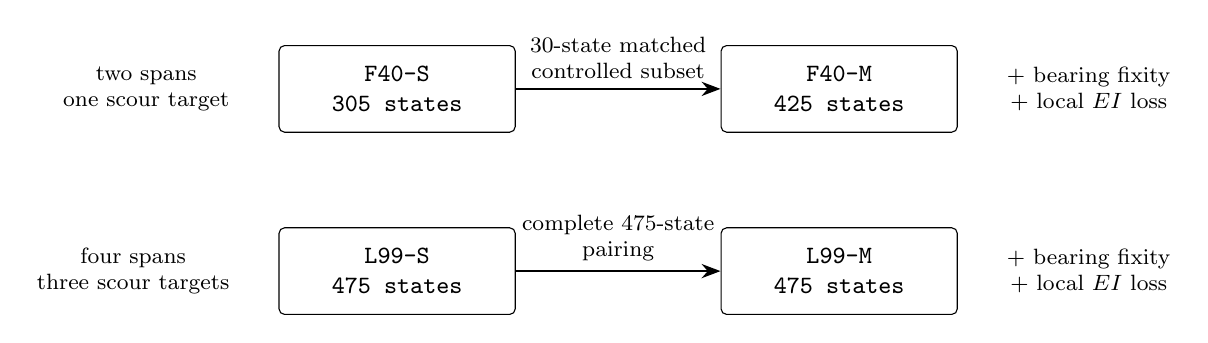
\begin{tikzpicture}[
  node distance=12mm and 26mm,
  block/.style={draw, rounded corners=2pt, minimum height=11mm,
    minimum width=30mm, align=center, font=\small\ttfamily},
  arr/.style={-{Stealth[length=2.4mm]}, thick},
  lbl/.style={font=\footnotesize, align=center}
]
\node[block] (f40s) {F40-S\\305 states};
\node[block, right=of f40s] (f40m) {F40-M\\425 states};
\draw[arr] (f40s) -- node[above,lbl] {30-state matched\\controlled subset} (f40m);
\node[block, below=of f40s] (l99s) {L99-S\\475 states};
\node[block, right=of l99s] (l99m) {L99-M\\475 states};
\draw[arr] (l99s) -- node[above,lbl] {complete 475-state\\pairing} (l99m);
\node[lbl, left=5mm of f40s] {two spans\\one scour target};
\node[lbl, left=5mm of l99s] {four spans\\three scour targets};
\node[lbl, right=5mm of f40m] {+ bearing fixity\\+ local $EI$ loss};
\node[lbl, right=5mm of l99m] {+ bearing fixity\\+ local $EI$ loss};
\end{tikzpicture}%
}
\caption{Four-block Paper-1 design. Arrows denote only authenticated semantic
state pairing; no causal or transport arrow connects the two geometries.}
\label{fig:stage_graph}
\end{figure}

\begin{table}[htbp]
\centering
\caption{Registered Paper-1 scientific blocks. Every state has 50 passages.
The profile is one fixed FRA-class-4 realization in all four blocks; speed,
temperature, and vehicle properties vary operationally.}
\label{tab:stages}
\small
\setlength{\tabcolsep}{4pt}
\begin{tabular}{llrlp{5.8cm}}
\toprule
Block & Geometry & States & Targets & Expressed bridge mechanisms \\
\midrule
\texttt{F40-S} & $2\times20$ m & 305 & support 2 & scour only; dense 61-severity $\times$ 5-replica grid \\
\texttt{F40-M} & $2\times20$ m & 425 & support 2 & scour + nominal bearing fixity + local $EI$ loss \\
\texttt{L99-S} & $4\times24.9$ m & 475 & supports 2--4 & multi-pier scour only \\
\texttt{L99-M} & $4\times24.9$ m & 475 & supports 2--4 & scour + nominal bearing fixity + local $EI$ loss \\
\bottomrule
\end{tabular}
\end{table}

Track-layer damage, wheel polygonization, and suspension damage remain present
in the single qualified source tree but are disabled by the four stage
configurations; no stripped scientific solver branch is used. Alternative
profile phases are also disabled. Their later
evaluation belongs to a separate track/train-damage study cut from the frozen
source revision; code availability is not evidence that those mechanisms were
active in Paper~1.

\subsection{Execution blocks and provenance}
\label{sec:blocks}

Each scientific block has its own authenticated generation contract,
hyperparameter studies, result manifests, and execution receipts. Within a
block, compared training arms use the same GPU model and pinned numerical
stack; physical host identity may differ only where the compatibility contract
permits it. Data generation may be distributed across independently qualified
hosts. Every reported row is bound to the generating source revision, channel
schema, protocol hashes, split identity, and artifact digests, so that a
result without a complete authenticated lineage fails closed rather than being
silently admitted.

\section{Numerical simulation}
\label{sec:simulation}

\subsection{Train--track--bridge interaction model}
\label{sec:ttbi}

Vehicle responses are generated with a two-dimensional, vertically coupled
train--track--bridge interaction (TTBI) model implemented in MATLAB and derived
from the TTB-2D/VEqMon2D framework of Cantero
\cite{cantero_ttb2d, cantero2022veqmon}. The model couples (i) an
Euler--Bernoulli multi-span deck on vertical support springs and abutment
rotational springs; (ii) a discrete layered track containing rail, pads,
sleepers, ballast, and sub-ballast; and (iii) five identical planar vehicles
with car-body and two-bogie vertical/pitch degrees of freedom and four
constrained unsprung wheelset masses. Vehicle properties follow the
implemented intercity-train calibration attributed to O'Brien et
al.~\cite{obrien2018vehicle}. Wheel--rail interaction is linear and bilateral.
The directly coupled equations are integrated by average-acceleration
Newmark-$\beta$ ($\gamma=1/2$, $\beta=1/4$) at 1~ms.

\paragraph{Implementation provenance.}
The generator is a modified derivative of the published TTB-2D v1 code line,
based on archived upstream commit \texttt{28d35528} and redistributed under
GPL-3.0. The damage mechanisms, campaign catalogues, serialization, and
qualification gates described here are repository-local additions and must not
be attributed to the upstream author. Likewise, the track-property file cites
Zhai et al.~\cite{zhai2004track} and the vehicle file cites O'Brien et
al.~\cite{obrien2018vehicle}; those citations establish the source files'
provenance, not independent validation of every transferred value or topology.

Two bridge geometries are used (Figure~\ref{fig:model}). \textbf{F40} has two
20~m spans and one scour target at the internal support. \textbf{L99} has four
24.9~m spans (99.6~m total) and targets at the three internal supports. The
adopted $E$, $I$, mass per unit length, and 3\% bridge-damping target originate
from the Fernandes two-span example; their use for L99 is an idealized
geometry/scale stress, not calibration of a 99.6~m field bridge. Every state
must pass the registered broad frequency gate and healthy states must reproduce
the nominal healthy first frequency (approximately 4.13~Hz for F40 and
2.75~Hz for L99) within the authorized acceptance bands.

\begin{figure}[htbp]
\centering
\framebox[0.95\linewidth]{\rule{0pt}{4.2cm}\parbox{0.9\linewidth}{\centering
\footnotesize Figure placeholder --- F40 and L99 decks on vertical support
springs, simplified layered track, five-vehicle train, and eight
\texttt{physical8\_v1} channels on the leading vehicle. Redraw from the
authorized implementation.}}
\caption{Two-dimensional TTBI model, bridge geometries, and candidate modeled
response channels.}
\label{fig:model}
\end{figure}

\subsubsection{Geometry-specific support-aligned meshes}
\label{sec:mesh}

The production meshes are not universally 0.30~m. F40 uses a 0.20~m deck mesh
(three elements per 0.60~m sleeper bay) and a 0.30~m rail mesh (two per bay), so
the internal support is exactly a deck node at 20.0~m. This is a
support-alignment correction to the Fernandes-derived 0.30~m benchmark density:
0.30~m does not divide 20 or 40~m. L99 uses 0.30~m for both deck and rail,
which places all 24.9~m-spaced supports on nodes. Positive support springs are
required to coincide with nodes to roundoff tolerance; they are never snapped
to a nearby grid location.

Production Rayleigh coefficients are recomputed from the first two elastic
modes of each realized bridge state. Mesh-refinement studies independently
recompute the modal references and coefficients on every grid and save the
resulting $\alpha$, $\beta$, and reference modes. A fixed-coefficient arm using
the healthy reference is a sensitivity, not the production closure. Because
the rail-damping matrix uses the corresponding bridge frequencies as its
references, a structural-stiffness intervention in production changes both the
assembled $K$ and Rayleigh-dependent $C$ matrices; it is not evidence that
physical damage itself changes damping.

\subsubsection{Finite rail-domain selection}
\label{sec:rail_clearance}

The finite rail domain was selected by the source-locked 18-case matrix recorded
in \nolinkurl{docs/evidence/paper1_model_form_freeze_20260809.json}. The
production decision identifier is
\nolinkurl{paper1-rail-domain-clearance-c06-v1}.
For each of F40 and L99, the matrix crossed three operating points
$(70~\mathrm{km/h},3\,^{\circ}\mathrm{C})$,
$(80~\mathrm{km/h},18\,^{\circ}\mathrm{C})$, and
$(90~\mathrm{km/h},33\,^{\circ}\mathrm{C})$ with 6, 15, and 30~m clearances.
All 18 cases completed. Both registered comparison tiers --- C06 versus C30
and C15 versus C30 --- passed, so the rule selected 6~m for production. The
verdict is bound to generator source-root SHA-256
\nolinkurl{aa187204cb3f89e24cb8bc894034044bad38b0358f5e0cd586338f84a8418efb}.
Its authorized claim is strictly finite-rail-domain selection for this
source-locked case matrix; it is not general mesh/time-step convergence,
damage-model validation, or physical/field validation.

\subsubsection{Track-property and topology boundary}
\label{sec:track_boundary}

The implemented nominal track is an inherited hybrid planar convention, not a
blanket sum of all Zhai quantities into two rails. Zhai et
al.~\cite{zhai2004track} report their Table~1 quantities per rail seat at
0.545~m spacing. The implementation doubles rail inertia and rail mass and uses
a full sleeper mass, but retains the tabulated pad, ballast, and sub-ballast
terms at one-seat values. It then places those values on a 0.600~m sleeper
lattice without re-evaluating the spacing-dependent $M_b$, $K_b$, and $K_f$
expressions. The production baseline is therefore neither a demonstrated
one-seat line model nor a consistently doubled two-rail equivalent.

The topology is also simplified relative to Zhai: adjacent-ballast shear
couplings $K_w,C_w$ are omitted, and the complete retained ballast mass is
condensed onto the support-aligned deck degree of freedom at every on-bridge
sleeper. This is an explicit inherited model-form choice. The topology arm was
dropped because it would require new solver structure and is not examined in
this paper.

Three parameter-level sensitivity families are prospectively fixed against the
hybrid baseline: (i) consistent one-seat and consistent two-rail scaling;
(ii) recomputation of $M_b$, $K_b$, and $K_f$ at 0.600~m from Zhai's equations;
and (iii) 0.050\% and 0.200\% rail-damping targets around the inherited 0.100\%
target. The 0.100\% target is author-chosen and is not reported by Zhai.
Sensitivity outcomes qualify interpretation but do not silently redefine the
production model after its source freeze.

\begin{table}[htbp]
\centering
\caption{Nominal physical and numerical parameters read from the implemented
baseline. Track entries preserve the hybrid scaling and topology described in
Section~\ref{sec:track_boundary}; they must not be labeled uniformly
``two-rail Zhai values''.}
\label{tab:parameters}
\footnotesize
\setlength{\tabcolsep}{4pt}
\resizebox{\textwidth}{!}{%
\begin{tabular}{llll}
\toprule
Subsystem & Parameter & Value & Units \\
\midrule
\multirow{8}{*}{Bridge}
 & spans (F40 / L99) & $2\times20$ / $4\times24.9$ & m \\
 & Young's modulus $E$ at 15\,$^{\circ}$C & $35\times10^{9}$ & N/m$^2$ \\
 & second moment of area $I$ & 0.33 & m$^4$ \\
 & mass per unit length & 9600 & kg/m \\
 & Rayleigh target, first two elastic modes & 3 & \% \\
 & healthy vertical support stiffness $k_{v,0}$ & $3.44\times10^{8}$ & N/m \\
 & free-rotation abutment baseline & 0 & N$\cdot$m/rad \\
 & healthy first frequency (F40 / L99) & $\approx4.13$ / $\approx2.75$ & Hz \\
\midrule
\multirow{8}{*}{Track}
 & rail bending stiffness $EI$ & $1.325\times10^{7}$ & N$\cdot$m$^2$ \\
 & rail mass (doubled-rail entry) & 121.28 & kg/m \\
 & rail Rayleigh target (inherited) & 0.100 & \% \\
 & pad stiffness / damping (one-seat entry) & $6.5\times10^{7}$ / $7.5\times10^{4}$ & N/m, N$\cdot$s/m \\
 & sleeper spacing / full mass & 0.600 / 251 & m, kg \\
 & ballast mass / stiffness / damping (one-seat entries) & 531.4 / $1.3775\times10^{8}$ / $5.88\times10^{4}$ & kg, N/m, N$\cdot$s/m \\
 & sub-ballast stiffness / damping (one-seat entries) & $7.75\times10^{7}$ / $3.115\times10^{4}$ & N/m, N$\cdot$s/m \\
 & finite rail clearance beyond deck & 6 & m \\
\midrule
\multirow{7}{*}{Vehicle ($\times5$)}
 & car-body mass / pitch inertia & 36852 / 560342 & kg, kg$\cdot$m$^2$ \\
 & bogie mass / pitch inertia & 3910 / 10024 & kg, kg$\cdot$m$^2$ \\
 & wheelset mass & 1407 & kg \\
 & primary suspension stiffness / damping per axle & $5.558\times10^{6}$ / $5.88\times10^{4}$ & N/m, N$\cdot$s/m \\
 & secondary suspension stiffness / damping per bogie & $2.0\times10^{6}$ / $1.2\times10^{5}$ & N/m, N$\cdot$s/m \\
 & bogie-centre / axle spacing & 16 / 2.3 & m \\
 & vehicle length / wheel radius & 22 / 0.46 & m \\
\midrule
\multirow{4}{*}{Solver}
 & integration & Newmark-$\beta$ ($\gamma=1/2$, $\beta=1/4$) & --- \\
 & time step / stored rate & $10^{-3}$ / 1000 & s, Hz \\
 & deck element (F40 / L99) & 0.20 / 0.30 & m \\
 & rail element (F40 / L99) & 0.30 / 0.30 & m \\
\bottomrule
\end{tabular}%
}
\end{table}

\subsection{Response-channel schema}
\label{sec:response_channels}

The leading vehicle supplies the eight candidates in
Table~\ref{tab:channels}, identified collectively as
\texttt{physical8\_v1}. Six are direct responses of modeled car-body/bogie
degrees of freedom. The other two are the total vertical accelerations implied
by the constrained motion of the first two wheelsets,
\begin{equation}
  \ddot z_w = u_{,tt} + 2v\,u_{,xt} + v^2 u_{,xx} + \ddot h_w,
  \label{eq:wheelset_proxy}
\end{equation}
where $u$ is the rail displacement field evaluated along the moving contact
coordinate, $v$ is passage speed, and $h_w$ is the prescribed profile/wheel
path. These two rows are idealized, model-predicted
\emph{constrained-wheelset acceleration proxies}. They are not independent
wheelset degrees of freedom, not the Eulerian rail-field acceleration
$u_{,tt}$ alone, and not validated measurements from axle-box sensors.
The separate stored \texttt{acc\_under} rows remain virtual rail-field
diagnostics and never enter the eight-channel screen.

\begin{table}[htbp]
\centering
\caption{Candidate \texttt{physical8\_v1} responses of the leading vehicle.}
\label{tab:channels}
\small
\begin{tabular}{cll}
\toprule
Index & Response channel & Observation status \\
\midrule
0 & car-body vertical acceleration & modeled secondary-suspended DOF \\
1 & front-bogie vertical acceleration & modeled primary-suspended DOF \\
2 & rear-bogie vertical acceleration & modeled primary-suspended DOF \\
3 & wheelset-1 constrained vertical acceleration & idealized total-motion proxy \\
4 & wheelset-2 constrained vertical acceleration & idealized total-motion proxy \\
5 & car-body pitch angular velocity & modeled secondary-suspended DOF \\
6 & front-bogie pitch angular velocity & modeled primary-suspended DOF \\
7 & rear-bogie pitch angular velocity & modeled primary-suspended DOF \\
\bottomrule
\end{tabular}
\end{table}

The proxy label is deliberate. Equation~\eqref{eq:wheelset_proxy} omits a
hardware observation chain, local axle-box mounting dynamics, sensor bandwidth
and filtering, and contact nonlinearity. Accordingly, the channel screen ranks
modeled responses and does not determine a transducer count or procurement
choice.

\subsubsection{Contact-model scope and qualification}
\label{sec:contact}

The bilateral linear contact model does not simulate separation and re-contact.
Wheel flats and polygonization are disabled in all four Paper-1 blocks. Every
retained passage nevertheless carries finite/contact diagnostics and fails
generation if it violates the registered admissibility contract. Before
dispatch, the contact-closure study evaluates all 420 passages of the four
marked qualification datasets at 1.0, 0.5, and 0.25~ms, applies the registered
0/12/24~kN tension gates and 0.002 path-fraction gate, and checks waveform and
quantity-of-interest convergence. This is an engineering consistency gate for
the finite design, not validation of bilateral contact physics.

\subsection{Active bridge mechanisms}
\label{sec:mechanisms}

\subsubsection{Scour as support-stiffness loss}
\label{sec:scour_mech}

At each target support, scour is represented as
\begin{equation}
  k_v(d)=(1-d)k_{v,0}, \qquad 0\le d\le0.60,
  \label{eq:scour}
\end{equation}
with $k_{v,0}=3.44\times10^8$~N/m. The regression label is $100d$,
modeled support-stiffness loss in percentage points. This follows the
drive-by-scour convention~\cite{fernandes2024driveby,
fernandes2025early, prendergast2013investigation}, but is not scour depth,
embedment loss, or eroded volume.

\subsubsection{Nominal bearing fixity}
\label{sec:bearing_mech}

F40-M and L99-M activate a rotational spring at each abutment. The sampled
geometry-normalized coordinate is
\begin{equation}
 \varphi=\frac{k_r}{k_r+4E_{15}I/L_{\mathrm{end}}}
 \quad\Longleftrightarrow\quad
 k_r=\frac{\varphi}{1-\varphi}\frac{4E_{15}I}{L_{\mathrm{end}}},
 \qquad \varphi\in[0,0.95].
 \label{eq:fixity}
\end{equation}
The stiffness is computed once using the fixed 15\,$^{\circ}$C modulus and
remains constant while the deck modulus varies between passages. The two
fixity coordinates are additional M-block regression targets. They are nominal
free-to-near-fixed design variables, not calibrated bearing-damage percentages
or physical seizure thresholds.

\subsubsection{Local flexural-rigidity-loss surrogate}
\label{sec:crack_mech}

F40-M and L99-M reduce $EI$ uniformly over the single production finite element
containing the sampled damage location, with author-chosen severity
$\mathcal{U}(0.05,0.30)$. Locations use an author-chosen 4:1 design weighting
toward hogging regions inside the registered support-zone and bridge-length
bounds. No fitting dataset supports those occurrence or severity laws. The
damaged length is consequently one mesh-locked element --- 0.20~m on F40 and
0.30~m on L99 --- rather than a common physical crack length. This is a local
damaged-element benchmark, not the tapered crack-depth model of Sinha et
al.~\cite{sinha2002simplified}; its severity is never interpreted as crack
depth. Crack status is logged but not predicted.

\subsection{Fixed profile, operational variability, and deferred mechanisms}
\label{sec:opvar}

Every state and passage in all four blocks uses one generated realization of
the implemented FRA-class-4 vertical-profile spectrum (registered phase seed
20260728). No measured profile, per-state phase variation, or per-passage
profile jitter is used. The fixed choice enables exact paired comparisons but
removes profile variability from the production EOV distribution.

Operational conditions do vary. Each state's 50 passages use a Latin
hypercube over speed 70--90~km/h and temperature 3--33~$^{\circ}$C, rounded to
integer values. Temperature changes the deck modulus through the registered
author-chosen law
\[
 E(T)=E_{15}\,[1-0.003(T-15)].
\]
For each passage and vehicle, car-body mass has a 10\% Gaussian coefficient of
variation and primary/secondary suspension stiffnesses each have 5\%. These
envelopes and laws were not fitted to a route, climate, or fleet population.

Track-layer damage (ballast patches, hanging sleepers, and pad failure), wheel
polygonization, suspension damage, and alternative rail-profile phases are
disabled by all four stage contracts. The corresponding code remains in the
single source tree for future work; it contributes no expressed physics or
random variability to Paper~1.

\subsection{State catalogues and common random numbers}
\label{sec:states}

Table~\ref{tab:families} gives the exact state inventories. F40-S is a dense
61-severity grid (0--60\% in one-percentage-point increments) with five
semantic replicas per severity. F40-M uses five controlled families. Its five
healthy replicas and five replicas at each of 12, 24, 36, 48, and 60\% scour
form the exact 30-state subset shared with F40-S. L99-S and L99-M share their
complete five-family, 475-state latent design; bearing/crack coordinates are
dormant in L99-S rather than being removed or redrawn.

\begin{table}[htbp]
\centering
\caption{Registered state families. Every state has 50 operational passages.}
\label{tab:families}
\small
\begin{tabular}{lrrrp{5.0cm}}
\toprule
Family & F40-S & F40-M & L99-S/M & Role \\
\midrule
\texttt{target\_healthy} & 5 & 50 & 50 & zero-scour diagnostic \\
\texttt{scour\_only} & 300 & 25 & 75 & controlled support/severity anchors \\
\texttt{bearing\_only} & 0 & 50 & 50 & bearing/leakage anchors; dormant in L99-S \\
\texttt{nuisance\_only} & 0 & 50 & 50 & local-$EI$ anchors; dormant in L99-S \\
\texttt{joint} & 0 & 250 & 250 & multivariate latent design \\
\midrule
Total & 305 & 425 & 475 & \\
\bottomrule
\end{tabular}
\end{table}

Each state has a collision-checked semantic \texttt{StateUID}. Named substreams
derive operational, crack, profile, track, and passage identities from that UID
rather than a mutable row number or parallel-execution order. Only streams for
expressed Paper-1 mechanisms influence the solve; disabled track/wheel
namespaces remain inert. States are the split and resampling clusters, and
their 50 passages are correlated repeated observations, not independent field
samples.

The generator stores raw noise-free histories, semantic identities, latent
design coordinates, operational draws, profile and model-form identifiers,
modal/Rayleigh records, contact diagnostics, crop metadata, and source-bound
fingerprints. Observation noise is added only by the authenticated learning
pipeline (Section~\ref{sec:preprocessing}).

\section{Data processing and learning methodology}
\label{sec:data_processing}

\subsection{From generated responses to model inputs}
\label{sec:preprocessing}

\paragraph{Time-to-space transformation.}
Raw time histories are linearly interpolated onto a uniform spatial grid of
100 samples per metre and cropped to the registered bridge-centred window.
Speed is constant within a passage, so the time--space map is affine. This
aligns each bridge support and its response signature at the same input
location despite passage-speed variation.

\paragraph{RAW and PAA representations.}
The factorial compares the cropped spatial sequence directly (RAW) with true
Piecewise Aggregate Approximation (PAA) to 512 segments
\cite{keogh2001dimensionality}. PAA partitions the sequence into equal-width
windows and replaces each by its mean, with fractional boundaries handled
exactly. It is therefore both a dimensionality-reduction and low-pass
compression front end. Its inclusion follows drive-by damage-classification
precedent~\cite{fernandes2025early}; no universal denoising advantage is
assumed. RAW and PAA use the same downstream model interfaces.

\paragraph{Observation-noise stress.}
The main observation arm adds pointwise zero-mean Gaussian multiplicative
noise with standard deviation $0.05|x|$ after the space transform and crop but
before PAA and scaling. The generator is keyed by global channel index, so a
channel receives the same noise realization when evaluated alone or in any
pair. This is a symmetric mathematical stress, not a sensor model: it contains
no transducer-specific noise density, bias, bandwidth, mounting transfer
function, or environmental qualification~\cite{en61373}.

\paragraph{Per-channel scaling.}
A per-channel affine standardization is fitted on training states only and
applied unchanged to validation and test data. Fold-level adjudication refits
the scaler within each fold-training partition. No scaler sees its validation
fold or the sealed outer test.

\subsection{Learning tasks}
\label{sec:task}

The primary task is continuous multi-output regression. F40-S and F40-M have
one scour head for support~2; L99-S and L99-M have one scour head for each of
supports 2--4. The M blocks additionally contain one nominal-fixity head for
each abutment. Scour targets span 0--60 percentage points and fixity targets
0--95. The M-block training loss is a range-normalized multi-head MSE with
weights proportional to the inverse squared target range and normalized to
mean one. Selection remains scour-primary; bearing error and
scour--bearing leakage are secondary diagnostics. F40-S also supplies a
predeclared four-class subset at 0, 5, 10, and 20\% modeled stiffness loss for
a secondary Fernandes-style comparability check.

\subsection{Factorial architecture grid}
\label{sec:architectures}

The architecture experiment is the complete
\[
  \{\mathrm{RAW},\mathrm{PAA}\}
  \times\{\mathrm{position\ off,on}\}
  \times\{\mathrm{LSTM\ off,on}\}
  \times\{\mathrm{multi\!\mbox{-}\!rate\ off,on}\},
\]
giving 16 cells. All cells share a one-dimensional convolutional backbone and
dense regression heads; the three binary components have these meanings:

\begin{itemize}
  \item \textbf{Time2Vec-style spatial-coordinate encoding.} One linear and
  seven learnable sinusoidal functions of normalized bridge position are
  concatenated to the input, following the Time2Vec construction
  \cite{kazemi2019time2vec} on a spatial rather than temporal coordinate. The
  implementation is not a full Space2Vec model~\cite{mai2020space2vec}.
  \item \textbf{LSTM recurrence.} A unidirectional LSTM
  \cite{hochreiter1997long} follows the convolutional backbone, motivated by
  CNN--LSTM precedent in drive-by scour classification
  \cite{fernandes2026canelas}.
  \item \textbf{Fixed-width multi-rate pooling.} Parallel adaptive temporal
  pyramid branches summarize several registered rates and concatenate a fixed
  number of features. The output width and dense parameter count do not depend
  on RAW/PAA sequence length. The module is inspired by the multi-rate idea in
  N-HiTS~\cite{challu2023nhits}, but it is not the N-HiTS forecasting
  architecture: it has no backcast/forecast stacks or hierarchical
  interpolation.
\end{itemize}

The cell with all three components off is the CNN--global-average-pooling
(CNN--GAP) baseline within each representation. The factorial estimates
matched finite-design component contrasts, but does not prove that a component
is universally beneficial outside the registered search spaces and budget.

\begin{figure}[htbp]
\centering
\framebox[0.95\linewidth]{\rule{0pt}{4.0cm}\parbox{0.9\linewidth}{\centering
\footnotesize Figure placeholder --- RAW/PAA processing followed by the
$2\times2\times2$ position/LSTM/fixed-width-multi-rate neural factorial and
multi-head regression.}}
\caption{Processing chain and 16-cell factorial architecture grid.}
\label{fig:architectures}
\end{figure}

\begin{table}[htbp]
\centering
\caption{Registered continuous hyperparameter-search domains shared across
eligible cells; conditional domains appear only when their component is on.}
\label{tab:search_space}
\small
\begin{tabular}{lll}
\toprule
Scope & Hyperparameter & Domain \\
\midrule
base & convolutional layers & integer 2--4 \\
base & dense layers & integer 1--3 \\
base & learning rate & log-uniform $10^{-4}$--$10^{-2}$ \\
base & weight decay & log-uniform $10^{-5}$--$10^{-3}$ \\
per convolution & filters / kernel / max-pooling & 16--128 step 16 / $\{2,3,5,7\}$ / off,on \\
per dense layer & units / dropout & 32--256 step 16 / 0.1--0.5 \\
LSTM on & layers / hidden width / dropout & 1--2 / 32--128 step 32 / 0.1--0.4 \\
multi-rate on & adaptive-pyramid rate set & $\{(1,2,4),(1,4,8),(1,3,6),(1,2,4,8)\}$ \\
\bottomrule
\end{tabular}
\end{table}

Every trial uses batch size 32, at most 50 epochs, early-stopping patience 5,
Adam~\cite{kingma2015adam}, and cosine learning-rate annealing
\cite{loshchilov2017sgdr}. Failed trials, retries, out-of-memory events, and
incomplete terminal accounting fail the publication contract.

\subsection{State-grouped split and sealed-test firewall}
\label{sec:split}

States, never passages, are assigned by semantic identity to a deterministic
60/20/20 train/inner-validation/outer-test split (outer split seed 42). All 50
passages of one state remain together. The replicated controlled cells allocate
their five semantic replicas 3/1/1 across the three partitions; joint-state
strata preserve registered severity and nuisance balance. The identical split
is used wherever a semantic state is paired across blocks. The outer test stays
sealed through factorial HPO, development adjudication, channel screening, and
selected-pair HPO.

\subsection{F40-S factorial HPO and Option-C adjudication}
\label{sec:hpo}

The prospectively chosen HPO input is channel~1, front-bogie vertical
acceleration. On F40-S, each of the 16 cells receives five independent Optuna
restarts~\cite{akiba2019optuna} of 100 trials with the registered TPE sampler
\cite{bergstra2011algorithms} and successive-halving pruner
\cite{jamieson2016non}: 80 studies and 8,000 requested trials.

The best vector from each restart is then adjudicated by Option~C on one
prospectively fixed grouped-development OOF partition (seed 271828,
$n_{\mathrm{splits}}=3$, one repeat). Every candidate is refitted on folds
0--2 with initialization seeds 424243 and 8675309. Thus each cell has
$5\times3\times2=30$ fits and the factorial has 480. For every
candidate/initialization pair, the three validation folds are disjoint and
cover each development state exactly once. Scour MSE is first averaged across
the two initialization seeds within each state and then equally across states.
The minimum selects the vector; an exact tie selects the lowest HPO-restart
seed. The best RAW and PAA cells are their respective minimum-score cells, with
lexicographic cell identifier as the tie-break. These 480 fits are a selection
mechanism, not a post-selection stability estimate.

Four pipeline slots are retained: the best RAW cell, the best PAA cell, and the
RAW and PAA CNN--GAP baselines. If a winner is its representation's baseline,
the authenticated alias is deduplicated rather than treated as an independent
pipeline.

\subsection{Prospectively fixed response-channel screen}
\label{sec:channel_design}

The F40-S screen uses the eight \texttt{physical8\_v1} channels in
Table~\ref{tab:channels}. For each retained slot, it evaluates all eight
singles and all $\binom{8}{2}=28$ ascending pairs at the adjudicated frozen
hyperparameters and checkpoint epoch, using paired initialization seeds
4001, 4003, 4007, 4013, and 4019. The prospectively enumerated grid therefore
contains $4\times36\times5=720$ job slots before authenticated alias
deduplication; a winner/baseline alias is not retrained as though it were a
distinct pipeline. Each fit uses the canonical train-to-inner-validation
grouped partition; the outer test remains sealed.

For one input/pipeline, per-state scour MSE is averaged over the five seeds and
then equally across validation states. The input score is then averaged equally
over unique resolved pipelines. Singles are reported diagnostics but cannot
select. The minimum among the 28 pairs wins, with lexicographic ascending-pair
tie-breaking. The artifact authenticates the full result tensor, state
coverage, and deduplication map; no result-dependent pair can be inserted.

\subsection{Selected-pair HPO, stability, and secondary transfer}
\label{sec:post_selection}

After pair selection, each of the four retained slots receives five new
100-trial searches on that pair in F40-S. The same four slots receive
independent five-by-100-trial selected-pair HPO in F40-M, L99-S, and L99-M.
This contributes another 80 studies and 8,000 requested trials. Together with
the factorial anchor, the registered HPO budget is exactly 160 studies and
16,000 trials. There is no transport gate, no rescue trigger, and no primary
downstream result based on inherited F40-S hyperparameters.

After each block's vectors and checkpoint policy are frozen, four slots are
trained on the complete development set with 30 disjoint prospectively listed
initialization seeds and evaluated on the sealed outer test: $4\times4\times
30=480$ report-only stability fits. They cannot re-rank the selected models.
A separate secondary analysis applies frozen F40-S settings to the three
downstream blocks with four slots and five seeds ($3\times4\times5=60$ fits).
It is descriptive/non-selection only. The complete prospective refit grid is
480 adjudication + 720 channel-screen + 480 stability + 60 transfer = 1,740
listed fits, subject only to authenticated alias deduplication.

\subsection{Evaluation and registered analyses}
\label{sec:metrics}

Primary block tables report scour MSE in squared percentage points, aggregate
and per support, with RMSE where useful. Multi-pier blocks additionally report
the passage-level most-affected-support localization accuracy for passages
whose maximum true scour is strictly above 5 percentage points. M blocks report
bearing-head MSE, false scour response in bearing-only states, and false
bearing response in scour-only states. Seed distributions and state-first
resampling summaries are reported as descriptive finite-design sensitivity,
not population confidence intervals.

The two paired S--M analyses use only identical sealed-test StateUIDs and a
fixed paired seed axis. Within a seed, scour MSE is averaged equally over
eligible states; the registered point statistic is the median across the finite
seed list. One hundred thousand paired state-first bootstrap draws (seed 42;
the seed axis is never resampled) provide a pointwise descriptive interval and
a wider two-comparison tail-adjusted envelope. Neither has population coverage
or familywise-error-control semantics. F40 uses its exact 30-state shared
subset; L99 uses all 475 shared states.

\subsection{Reproducibility and provenance}
\label{sec:reproducibility}

Generation is bound to a registered MATLAB numerical-stack descriptor and
learning to a pinned Python/PyTorch/CUDA environment. Source roots, generation
contracts, channel schema, split identity, study identities, weights, scalers,
selection artifacts, and execution receipts are content authenticated and
cross-checked at resume and analysis boundaries. Before dispatch, every
generation host must produce all four marked qualification micro-datasets;
every passage enters the cross-host comparison, and the designated contact
gate covers all 420 qualification passages. Training hosts must additionally
pass genuine RAW benchmark/capacity authorization. These checks provide
artifact integrity and internal consistency under a trusted-operator model;
they are not cryptographic hardware attestation.

\section{Results and discussion}
\label{sec:results}

% =====================================================================
% HARD RULE (do not remove until the campaign is complete):
% Populate this section ONLY from authenticated outputs of the complete
% four-block Paper-1 campaign at the clean campaign source commit. No number,
% figure, ranking, or qualitative outcome from a pilot or superseded design is
% admissible, even as a placeholder.
% =====================================================================

\subsection{Campaign accounting and local qualification}
\label{sec:accounting}

This subsection will identify the campaign source revision, protocol and
source-root digests, recorded generation and training environments, per-PC
capability/physics-smoke and CUDA-capacity results, rail-clearance and
response-sensitivity verdicts, contact/time-step closure, and exact artifact
inventories. It will
confirm 305/425/475/475 states and 50 passages per state for
F40-S/F40-M/L99-S/L99-M, respectively, and document that no failed, incomplete,
retried, out-of-memory, provenance-inconsistent, or post-contact-violation job
entered a reported result.
\pending{Complete accounting from the authenticated campaign artifacts,
including all 160 primary HPO studies, 1,440 planned primary refits, and
sealed-test openings.}

\subsection{F40-S architecture-factorial adjudication}
\label{sec:factorial_results}

The F40-S front-bogie anchor table will report all 16 registered
RAW/PAA$\times$position-encoding$\times$LSTM$\times$multi-rate cells. For each
cell, five 100-trial HPO winners are adjudicated by one complete three-fold
grouped-development OOF partition and two initialization seeds. Tables will
show the paired state-clustered OOF scour MSE used for selection, the selected
restart vector, and the best RAW and PAA cells. Outer-test values are excluded
from these selection tables by construction.
\pending{Authenticated 16-cell Option-C OOF table and selected RAW/PAA cells;
report ties using the prospectively fixed restart-seed and cell-ID rules.}

\subsection{Response-channel screen and selected pair}
\label{sec:selection_results}

For each of the four retained slots --- best RAW, best PAA, RAW CNN--GAP, and
PAA CNN--GAP, with authenticated alias deduplication --- the frozen F40-S
screen uses five paired initialization seeds. The eight-response payload is
retained, but wheelset
proxy indices 3 and 4 are diagnostic-only and never enter a fit. The eligible
screen therefore contains six non-selectable singles and 15 selection-eligible
pairs. Pair selection averages state-level scour MSE across seeds, validation
states, and unique resolved pipelines, with lexicographic ascending-pair
tie-breaking. The full tensor, coverage, and deduplication map will accompany
the selected pair.
\pending{Authenticated 420-job channel-screen table, single-channel diagnostics,
resolved-pipeline map, and selected physical two-channel pair.}

\subsection{Block-local selected-pair performance and stability}
\label{sec:block_results}

The selected pair is re-optimized for the four retained slots in F40-S and
independently in F40-M, L99-S, and L99-M. Primary tables will report scour MSE
in squared percentage points (aggregate and per support, with RMSE where
useful), post-freeze distributions across 30 disjoint initialization seeds per
slot and block, and the prospectively frozen comparator set. These 480
sealed-test stability fits are report-only: they cannot change a selected
pipeline, pair, hyperparameter vector, or checkpoint policy.
\pending{Authenticated block-local HPO winners and sealed-test estimates for
the resolved RAW/PAA winners and CNN--GAP baselines in all four blocks.}

Any secondary contemporary-architecture results are admitted only after this
screen and use the exact authenticated primary F40-S pair. ModernTCN- and
TSLANet-inspired challengers have no independent pair-selection path and cannot
change the primary factorial, screen, or selected pair.

\subsection{Multi-pier estimation, localization, and bearing leakage}
\label{sec:multipier_results}

For L99-S and L99-M, results will separate aggregate from support-specific
scour error and report parity plots for supports 2--4. Most-affected-support
localization is the registered passage-level estimate restricted to passages
whose maximum true scour exceeds 5 percentage points. For F40-M and L99-M,
bearing-head error, false scour response in bearing-only states, and false
bearing response in scour-only states will be reported separately from scour
performance.
\pending{Per-support estimation, localization, bearing-head, and
scour--bearing leakage results from authenticated sealed-test artifacts.}

\subsection{Paired S--M comparisons}
\label{sec:paired_results}

The two registered cross-block comparisons have different pairing scopes.
F40-S versus F40-M uses only their 30 shared controlled semantic states;
L99-S versus L99-M uses all 475 shared states. In each case the S--M change
jointly activates nominal bearing-fixity physics, local $EI$ loss, and bearing
heads/multi-task learning, so it is reported as a combined model/task contrast,
not an isolated bearing or crack effect. State-first paired summaries use only
authenticated shared identities and preserve the finite-design, descriptive
claim boundary.
\pending{Authenticated F40 and L99 paired S--M effects with explicitly
descriptive finite-design uncertainty summaries.}

\subsection{F40 classification comparability check}
\label{sec:classification_results}

The F40-S regression dataset also supplies the predeclared 0, 5, 10, and 20\%
severity subset used for a Fernandes-style classification comparability check.
With five semantic replicas per class, this arm is deliberately secondary and
is not treated as a headline estimate or an exact replication.
\pending{Authenticated classification-comparability results and their deviation
statement; do not import published targets as observed results of this study.}

\subsection{Model-form sensitivities}
\label{sec:model_form_results}

Before physical interpretation, the manuscript will report the prospective
one-seat/two-rail parameter scaling, 0.545-to-0.600~m spacing recalculation,
rail-damping-target, and fixed-healthy-Rayleigh sensitivities. The inherited
ballast-shear/condensation topology has no sensitivity arm and remains an
explicit limitation. These analyses qualify the model form; they do not select
the neural architecture or admit a new production configuration after freeze.
\pending{Authenticated model-form sensitivity estimates and the resulting
pre-freeze production verdicts.}

\subsection{Secondary frozen transfer}
\label{sec:transfer_results}

F40-S settings are additionally evaluated without block retuning on each of
the three downstream blocks for four slots and five initialization seeds (60
fits). These rows are descriptive, labeled secondary/non-selection, and kept
separate from the independently tuned primary block results.
\pending{Authenticated secondary frozen-transfer results, reported without a
transport or rescue claim.}

\subsection{Discussion}
\label{sec:discussion}

The discussion will be limited to authenticated estimates. It will address
whether RAW or PAA and each factorial component changes observed error under
the matched search budget; which eligible modeled-DOF response pair the F40-S
screen selects and what the diagnostic-only wheelset-proxy boundary implies;
whether the
four retained pipelines behave consistently after independent block-local
tuning; how multi-pier and bearing-aware tasks change errors; and how sensitive
the interpretation is to the registered track/damping model-form choices.
Cross-geometry patterns and frozen transfer will remain descriptive, and no
result will be generalized to field sensors, unseen profiles, or deferred
track/train damage.
\pending{Discussion grounded only in authenticated four-block estimates.}

\section{Limitations and practical feasibility}
\label{sec:limitations}

The claims supported by this study are bounded by its physical model,
observation model, and finite registered design. We state those boundaries
explicitly before discussing field deployment.

\subsection{Physical model and label semantics}

\begin{itemize}
  \item \textbf{Simulation only.} All responses are generated by the registered
  TTBI model; no field measurement enters the study. Every conclusion is
  conditional on this simulated distribution.

  \item \textbf{Two-dimensional vertical dynamics.} The model captures
  vertical and pitch response only. Lateral, torsional, soil-continuum, and
  pier-tilt behaviour --- all potentially informative for scour --- are absent.

  \item \textbf{The support spring is not soil--structure interaction.} One
  vertical spring per bridge support represents the foundation. The target is
  modeled support-stiffness loss in percentage points, not scour depth,
  embedment loss, or eroded volume; no universal hydraulic-to-stiffness mapping
  is claimed.

  \item \textbf{Bearing and crack labels are design coordinates.} Nominal
  abutment rotational fixity is not a calibrated physical bearing-condition
  percentage. The crack arm is a uniform local finite-element $EI$ reduction,
  not a breathing crack or calibrated crack-depth model
  \cite{sinha2002simplified}.

  \item \textbf{Fixed profile and restricted nuisance scope.} One generated
  FRA-class-4 profile realization is shared by every state and passage. Rail
  profile is therefore not an operational EOV in Paper~1, and no claim of
  transport to another track section is available. Track-layer damage, wheel
  polygonization, and suspension damage are disabled. Evaluating the frozen
  models later under varied profile phases would be a distribution-shift
  experiment, not robustness to an EOV represented during training.

  \item \textbf{The nominal track is an inherited simplified topology.} The
  planar source combines two-rail quantities for rail inertia/mass and a full
  sleeper, but retains other values that Zhai et al.~\cite{zhai2004track}
  report per rail seat. It also retains source values derived at 0.545~m on a
  0.600~m support lattice, omits the adjacent-ballast $K_w,C_w$ shear branch,
  and condenses each on-bridge ballast lump onto the support-aligned deck node.
  The production baseline is therefore neither a demonstrated one-seat model
  nor a consistently doubled two-rail model, and it is not a complete Zhai
  reproduction. Prospective one-seat/two-rail and 0.545-to-0.600~m
  parameter-transfer sensitivities quantify two parameter-level choices; the
  omitted-shear/condensation topology itself remains unexamined. If a wheelset
  proxy wins the channel selection, that topology limitation must be resolved
  before publication or the wheelset result cannot be headlined.

  \item \textbf{Damping is model-form dependent.} The 0.1\% rail Rayleigh
  target is an inherited author-chosen value, not a property reported by Zhai;
  a prospective damping sensitivity bounds that choice. Production recomputes
  bridge coefficients for each realized state and recomputes them separately
  on every mesh in refinement studies, with rail damping referenced to the
  corresponding bridge modes. A fixed-healthy/fixed-grid coefficient arm is a
  model-form sensitivity. Consequently, stiffness interventions in the
  production model alter both assembled stiffness and Rayleigh-dependent
  damping; they are not evidence for physical damage-dependent damping.

  \item \textbf{Bilateral contact.} The linear wheel--rail model does not
  simulate separation and re-contact. The authenticated contact gate aborts
  generation on registered violations, but passing that gate does not quantify
  the response error caused by the bilateral approximation.

  \item \textbf{Author-chosen operational design.} The speed and temperature
  envelopes, deck-modulus temperature law, and vehicle-property perturbations
  were not fitted to a route, climate, or fleet population. Results are
  conditional on those finite design choices.
\end{itemize}

\subsection{Observation model and channel-level claims}

\begin{itemize}
  \item \textbf{Noise is a symmetric stress, not a hardware model.} The 5\%
  relative-noise arm applies the same mathematical rule to every channel and
  includes no transducer noise density, bias stability, bandwidth, mounting
  transfer function, or environmental qualification.

  \item \textbf{Channels are not sensors.} The experiment ranks modeled
  responses, not physical transducer counts or placements. In particular, the
  two \texttt{physical8\_v1} wheelset rows are total constrained-motion
  acceleration proxies assembled from the linear model. They omit axle-box
  mounting dynamics, local wheel/rail compliance beyond the model, sensor
  bandwidth and filtering, and contact nonlinearity. They must not be described
  as measured axle-box accelerations without a separate observation model.
\end{itemize}

\subsection{Statistical scope}

\begin{itemize}
  \item \textbf{Conditional finite-budget selection.} ``Best'' means best
  under the registered 16-cell search space, HPO budgets, fixed folds, seed
  lists, and F40-S channel screen. Equal budgets do not eliminate finite-search
  optimization error, and no global architecture or sensor optimum is claimed.

  \item \textbf{Development adjudication is selection, not stability.} The
  480 Option-C out-of-fold fits choose the F40-S vectors and therefore cannot
  estimate post-selection stability. Stability is reported separately from 30
  disjoint post-freeze initialization seeds per retained pipeline and block on
  the sealed outer test; those runs cannot re-rank a model.

  \item \textbf{The channel screen has an asymmetric role.} Eight singles are
  reported but non-selectable; only the 28 pairs can win. Subsequent HPO on the
  selected pair may improve its block-local model but is not evidence that the
  pair beats the 27 pairs that were screened under frozen F40-S settings.

  \item \textbf{Descriptive uncertainty, not population coverage.} State-first
  resampling and across-seed summaries are finite-design sensitivity analyses.
  They are not confidence intervals for a field population, familywise-error
  controlled tests, or significance/superiority guarantees.

  \item \textbf{Independent tuning changes the cross-block estimand.} Primary
  results compare pipelines after block-local HPO. They do not estimate
  zero-shot transfer. Frozen F40-S settings are evaluated downstream only in a
  separately labelled, secondary non-selection analysis.

  \item \textbf{No detection claim.} The study reports continuous regression
  error and localization. Sensitivity, specificity, probability of detection,
  calibrated damage probability, and minimum detectable severity would require
  a development-selected decision threshold that this protocol does not define.
\end{itemize}

\subsection{Practical feasibility and implementation challenges}

Field use first requires a hardware-specific observation model. Transducers,
mounts, acquisition chains, and environmental loads differ markedly across a
vehicle; axle-box environments are especially demanding~\cite{en61373}.
Second, supervised deployment requires trustworthy labels or a credible route
through model updating, domain adaptation, or hybrid physics--data methods.
The simulation-to-field gap --- model-form error, unmodeled EOVs, traffic
variability, and asset variability --- remains the dominant unquantified risk
\cite{malekjafarian2015review, fernandes2026canelas}. Third, the spatial
transform assumes known passage speed and repeated passages require fleet and
positioning integration. Finally, the models cover one train class and two
idealized bridge geometries. Transfer across vehicles, bridge types, profiles,
and speeds outside 70--90~km/h is untested. A staged pathway should therefore
begin with instrumented healthy crossings for EOV and observation-model
calibration, followed by controlled stiffness interventions or monitored
scour-critical structures.

\section{Conclusion}
\label{sec:conclusion}

This paper established a prospectively specified, source-locked framework for
pre-deployment design of drive-by railway-bridge scour monitoring. The design
asks which RAW/PAA processing and neural components are useful, which pair of
modeled vehicle-response channels should be retained, how accurately one
passage can estimate several pier-specific support-stiffness-loss targets, and
how performance changes when nominal bearing fixity and a local
flexural-rigidity-loss surrogate are added to the task.

The framework's defining safeguards are four explicit scientific blocks
(F40-S, F40-M, L99-S, and L99-M); semantic state grouping and authenticated
common-random-number pairing only where the catalogues actually overlap; a
sealed outer test; Option-C grouped-development out-of-fold adjudication; a
prospectively fixed channel screen; independent selected-pair hyperparameter
optimization in every block; and a disjoint, report-only post-freeze stability
set. The earlier transport/rescue policy is not part of the experiment.
Track-layer damage, wheel polygonization, suspension damage, and alternative
rail-profile phases are likewise deferred rather than silently treated as
active. One generated FRA-class-4 profile realization is shared by every state
and passage.

The physical claim boundary is equally important. The primary label is modeled
vertical support-stiffness loss, not scour depth; bearing fixity is a nominal
design coordinate; the crack is a local $EI$-loss surrogate; and the two
wheelset rows in \texttt{physical8\_v1} are idealized constrained-motion
acceleration proxies, not validated axle-box sensor observations. They remain
diagnostic payload rows and are excluded from learning and channel selection;
the eligible screen contains six singles and 15 pairs. Optional contemporary
challengers enter only after that screen and use exactly the authenticated
primary F40-S pair.

\pending{Summarize only authenticated four-block outcomes: the RAW/PAA
factorial winners, selected physical channel pair, block-local sealed-test
performance and stability, multi-pier localization, bearing leakage, and the
two registered S--M paired comparisons.}

Within those boundaries, the study is designed to provide auditable answers
conditional on the simulated distribution. Field validation remains the
essential next step: the selected configurations must be confronted with
measured crossings, hardware-specific observation models, varied track
profiles, and the simulation-to-field gap that no simulation study can close
from within.


\section*{Acknowledgments}
% TBD: advisors (UFSC / UCSD), computing resources, discussion partners.

\subsection*{Author Contributions}
% TBD.

\subsection*{Funding}
% TBD (e.g., CAPES/CNPq sandwich scholarship --- fill in the grant program and number).

\subsection*{Conflicts of Interest}
The author(s) declare(s) that there is no conflict of interest regarding the
publication of this article.

\subsection*{Data Availability}
% Registered plan: release the campaign manifests (protocol descriptors, split
% manifests, HPO/champion manifests, execution receipts) and the analysis
% tables alongside the code repository; raw MATLAB time histories available on
% request due to size. Fill in the archive DOI at submission.
\pending{data archive DOI and released-artifact list}

\printbibliography

\end{document}
